HTTPS stands for Hypertext Transfer Protocol Secure.
HTTPS is an extension of the Hypertext Transfer Protocol.
It is used for secure communication over a computer network,
and is widely used on the Internet [\cite{lam2000secure, karayiannis2019implementing}].
In HTTPS, the communication protocol is encrypted using Transport Layer Security [\cite{turner2014transport}]
or, formerly, Secure Sockets Layer [\cite{weaver2006secure}].
The protocol is therefore also referred to as HTTP over TLS or HTTP over SSL\@.
The principal motivations for HTTPS are authentication of the accessed website, and protection of the privacy and integrity
of the exchanged data while in transit.
It protects against \textit{man-in-the-middle attacks}.
The bidirectional encryption of communications between a client and server protects the communications against
eavesdropping and tampering [\cite{mayer2016tlscompare, jiang2019physical}].
The authentication aspect of HTTPS requires a trusted third party to sign server-side digital certificates.
This was historically an expensive operation, which meant fully authenticated HTTPS connections were usually found only
on secured payment transaction services and other secured corporate information systems on the World Wide Web.
In 2016, a campaign by the Electronic Frontier Foundation with the support of web browser developers led to the protocol
becoming more prevalent [\cite{he2014shadowcrypt}].
HTTPS is now used more often by web users than the original non-secure HTTP, primarily to protect
page authenticity on all types of websites;
secure accounts;
and to keep user communications, identity, and web browsing private [\cite{rescorla2000rfc2818}].

\subsection{What is an SSL Certificate?}\label{subsec:what-is-an-ssl-certificate?}
SSL certificates are what enable websites to move from HTTP to HTTPS, which is more secure.
An SSL certificate is a data file hosted in a website's origin server.
SSL certificates make SSL/TLS encryption possible, and they contain the website's public key and the website's identity,
along with related information.
Devices attempting to communicate with the origin server will reference this file to obtain the public key and verify
the server's identity.
The private key is kept secret and secure.
SSL certificates include:
\begin{itemize}
    \item The domain name that the certificate was issued for
    \item Which person, organization, or device it was issued to
    \item Which certificate authority issued it
    \item The certificate authority's digital signature
    \item Associated sub-domains
    \item Issue date of the certificate
    \item Expiration date of the certificate
    \item The public key (the private key is kept secret)
\end{itemize}
The public and private keys used for SSL are essentially long strings of characters used for encrypting and decrypting data.
Data encrypted with the public key can only be decrypted with the private key, and vice versa.
\begin{figure}[H]
    \centering
    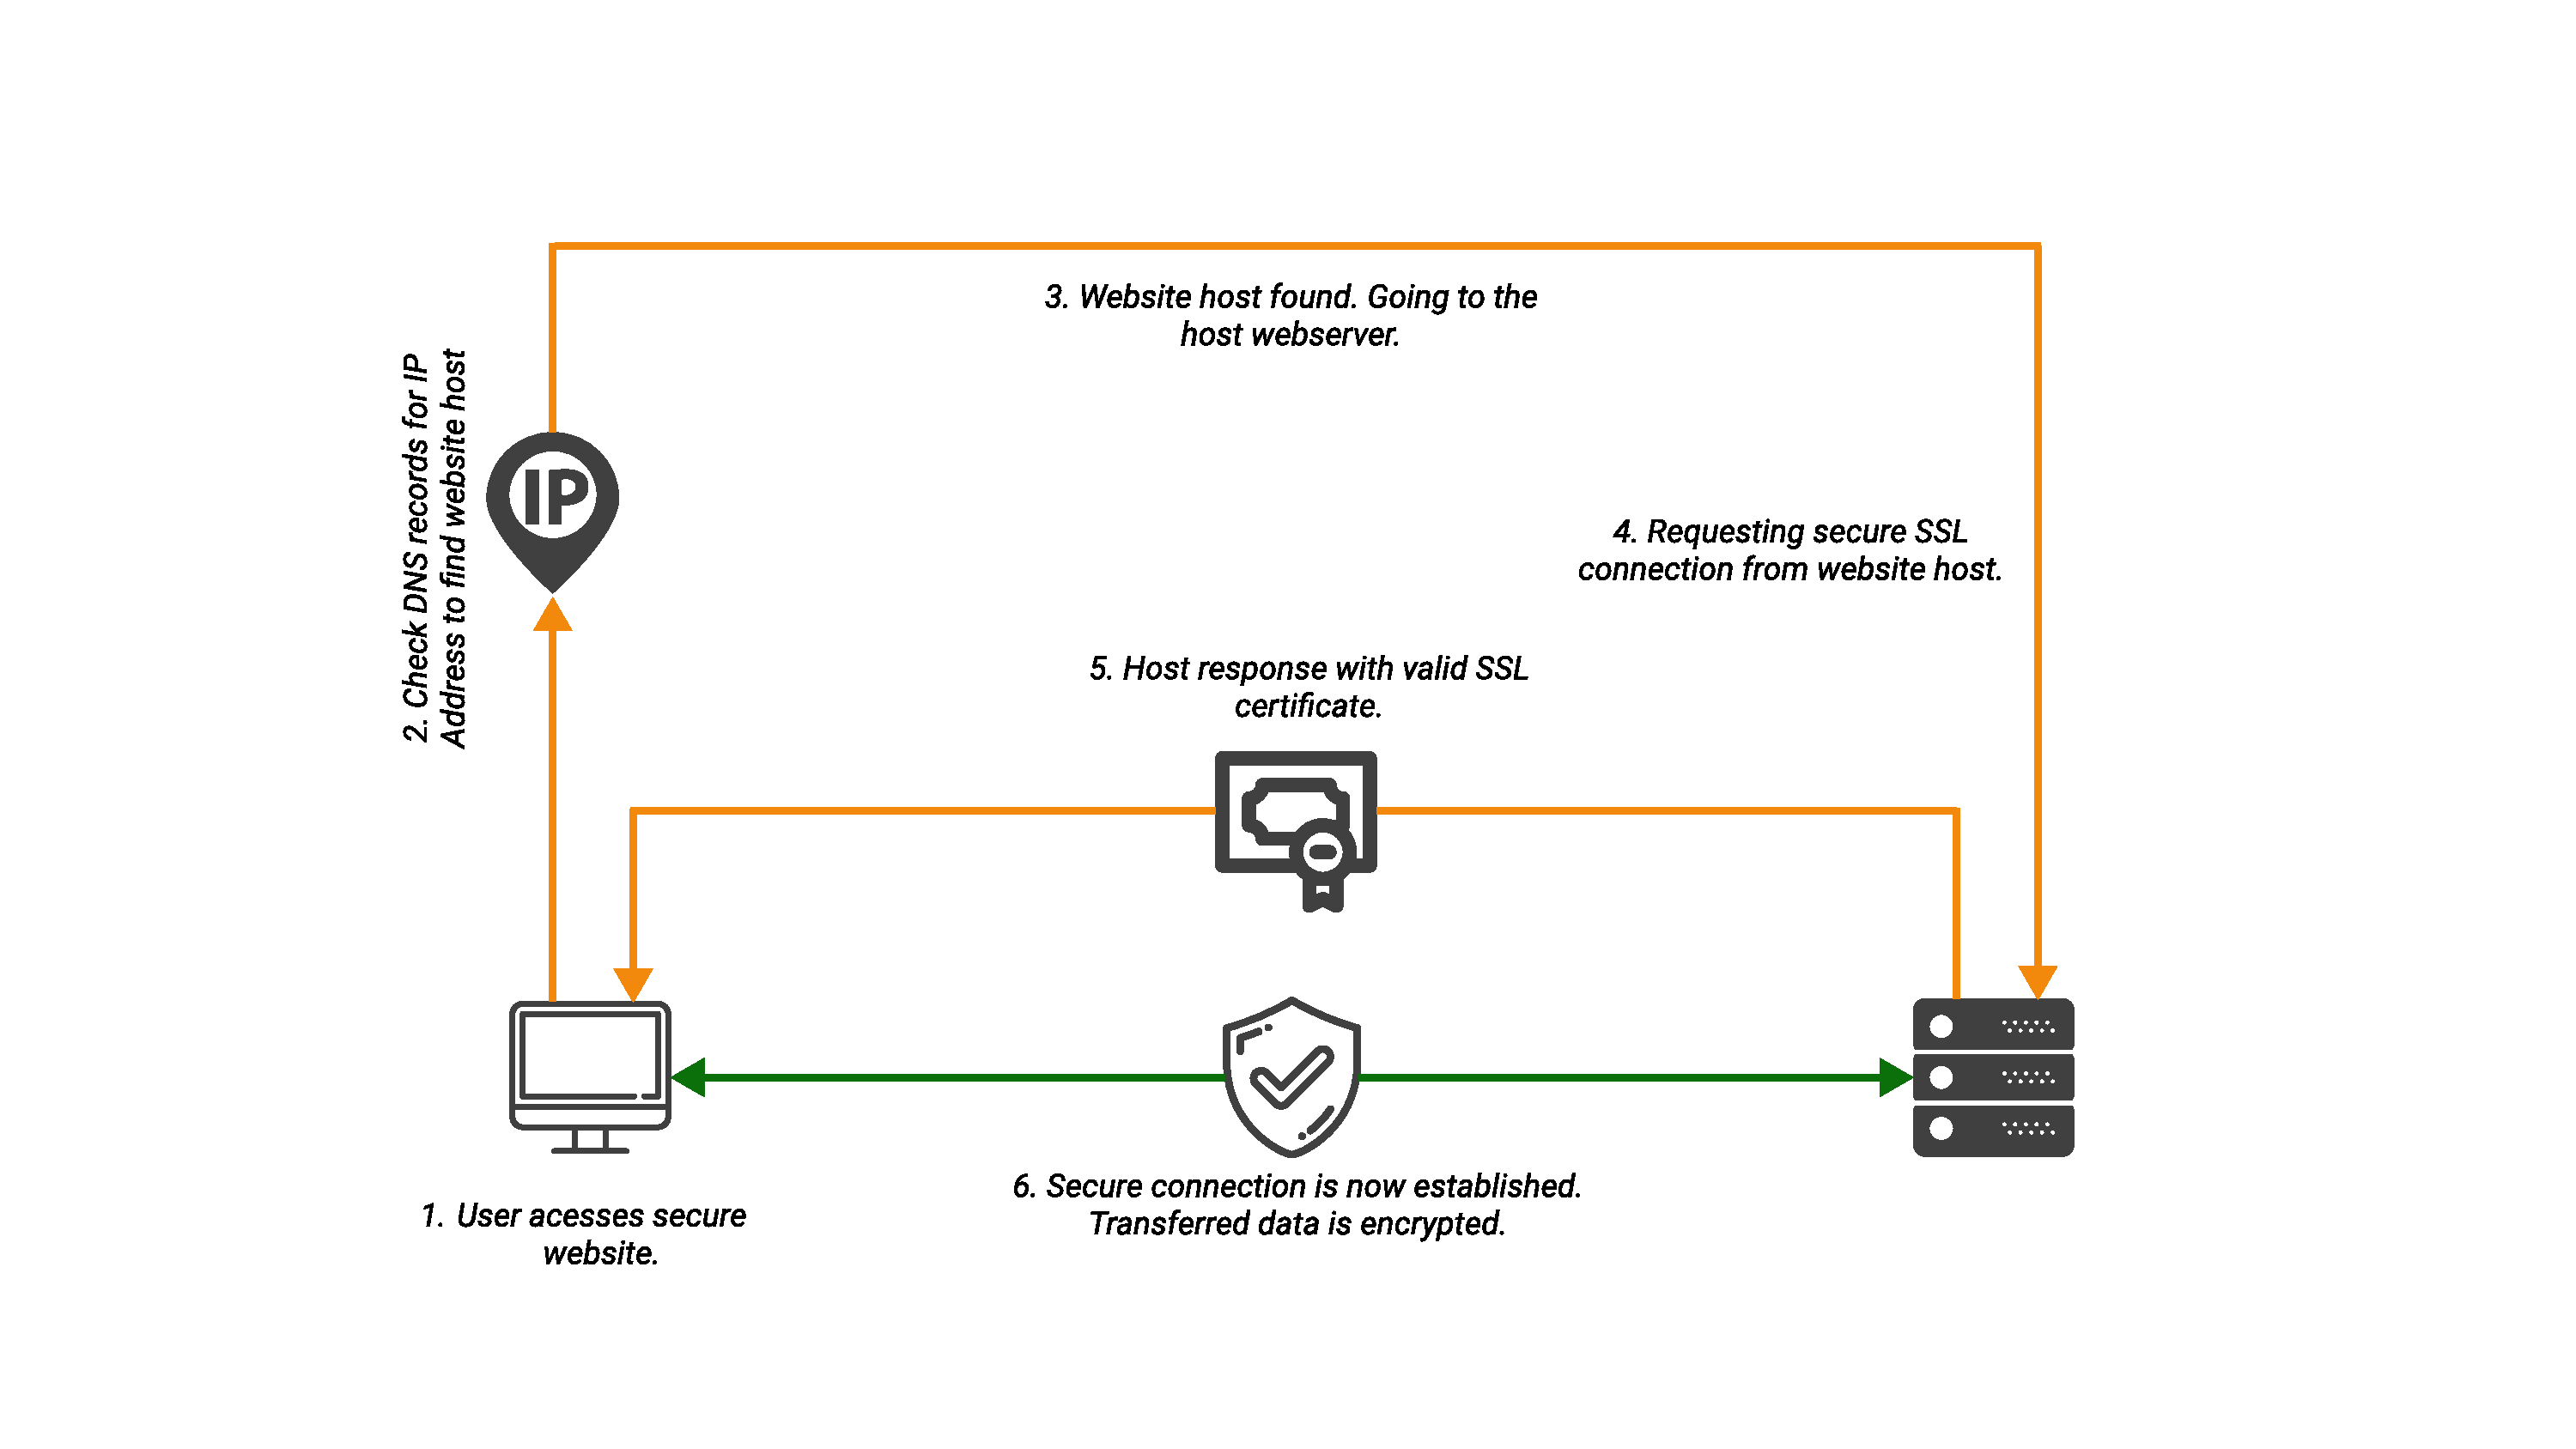
\includegraphics[width=1\textwidth]{Pictures/HTTPS_Flow}
    \caption{HTTPS flow diagram.}\label{fig:figure6}
\end{figure}

\subsection{Discussion on E2E Encryption over HTTPS Protocol}\label{subsec:discussion-on-e2e-encryption-over-https-protocol}
Discuss here about why it is useless to implement E2E encryption in web version,
however is ok to implement for mobile one [\cite{JsMathRandom, E2eVsTLS}].
Answer the questions:
\begin{itemize}
    \item What is End-to-End (E2E) Encryption?
    \item How it is used in telegram?
    \item Does it make sense to implement it for web version?
    \item Does it make sense to implement it for mobile version?
    \item Why is it not worth that to implement E2E for web version?
\end{itemize}